\documentclass[11pt,a4paper]{article}
%%%%%%%%%%%%%%%%%%%%%%%%% Credit %%%%%%%%%%%%%%%%%%%%%%%%

% template ini dibuat oleh martin.manullang@if.itera.ac.id untuk dipergunakan oleh seluruh sivitas akademik itera.

%%%%%%%%%%%%%%%%%%%%%%%%% PACKAGE starts HERE %%%%%%%%%%%%%%%%%%%%%%%%
\usepackage{graphicx}
\usepackage{caption}
% \usepackage{microtype} % Disabled to avoid font expansion errors
\captionsetup[table]{name=Tabel}
\captionsetup[figure]{name=Gambar}
\usepackage{tabulary}
\usepackage{minted}
\usepackage{amsmath}
\usepackage{fancyhdr}
\usepackage{amssymb}
\usepackage{amsthm}
\usepackage{placeins}
\usepackage{amsfonts}
\usepackage{graphicx}
\usepackage[all]{xy}
\usepackage{tikz}
\usepackage{verbatim}
\usepackage[left=2cm,right=2cm,top=3cm,bottom=2.5cm]{geometry}
\usepackage{hyperref}
\hypersetup{
    colorlinks,
    linkcolor={red!50!black},
    citecolor={blue!50!black},
    urlcolor={blue!80!black}
}
\usepackage{caption}
\usepackage{subcaption}
\usepackage{multirow}
\usepackage{psfrag}
\usepackage[T1]{fontenc}
\usepackage[scaled]{beramono}
% Enable inserting code into the document
\usepackage{listings}
\usepackage{xcolor} 
% custom color & style for listing
\definecolor{codegreen}{rgb}{0,0.6,0}
\definecolor{codegray}{rgb}{0.5,0.5,0.5}
\definecolor{codepurple}{rgb}{0.58,0,0.82}
\definecolor{backcolour}{rgb}{0.95,0.95,0.92}
\definecolor{LightGray}{gray}{0.9}
\lstdefinestyle{mystyle}{
	backgroundcolor=\color{backcolour},   
	commentstyle=\color{green},
	keywordstyle=\color{codegreen},
	numberstyle=\tiny\color{codegray},
	stringstyle=\color{codepurple},
	basicstyle=\ttfamily\footnotesize,
	breakatwhitespace=false,         
	breaklines=true,                 
	captionpos=b,                    
	keepspaces=true,                 
	numbers=left,                    
	numbersep=5pt,                  
	showspaces=false,                
	showstringspaces=false,
	showtabs=false,                  
	tabsize=2
}
\lstset{style=mystyle}
\renewcommand{\lstlistingname}{Kode}
%%%%%%%%%%%%%%%%%%%%%%%%% PACKAGE ends HERE %%%%%%%%%%%%%%%%%%%%%%%%


%%%%%%%%%%%%%%%%%%%%%%%%% Data Diri %%%%%%%%%%%%%%%%%%%%%%%%
\newcommand{\student}{\textbf{Ferdana Al-Hakim (122140012)}}
\newcommand{\course}{\textbf{Sistem Teknologi Multimedia (IF25-40305)}}
\newcommand{\assignment}{\textbf{Worksheet 1: Setup Python Environment untuk Multimedia}}

%%%%%%%%%%%%%%%%%%% using theorem style %%%%%%%%%%%%%%%%%%%%
\newtheorem{thm}{Theorem}
\newtheorem{lem}[thm]{Lemma}
\newtheorem{defn}[thm]{Definition}
\newtheorem{exa}[thm]{Example}
\newtheorem{rem}[thm]{Remark}
\newtheorem{coro}[thm]{Corollary}
\newtheorem{quest}{Question}[section]
%%%%%%%%%%%%%%%%%%%%%%%%%%%%%%%%%%%%%%%%
\usepackage{lipsum}%% a garbage package you don't need except to create examples.
\usepackage{fancyhdr}
\pagestyle{fancy}
\lhead{Ferdana Al Hakim (122140012)}
\rhead{ \thepage}
\cfoot{\textbf{Worksheet 1: Setup Python Environment untuk Multimedia}}
\renewcommand{\headrulewidth}{0.4pt}
\renewcommand{\footrulewidth}{0.4pt}

%%%%%%%%%%%%%%  Shortcut for usual set of numbers  %%%%%%%%%%%

\newcommand{\N}{\mathbb{N}}
\newcommand{\Z}{\mathbb{Z}}
\newcommand{\Q}{\mathbb{Q}}
\newcommand{\R}{\mathbb{R}}
\newcommand{\C}{\mathbb{C}}
\setlength\headheight{14pt}

%%%%%%%%%%%%%%%%%%%%%%%%%%%%%%%%%%%%%%%%%%%%%%%%%%%%%%%555
\begin{document}
\thispagestyle{empty}
\begin{center}
	
\includegraphics[scale = 0.15]{figure/ifitera-header.png}
	\vspace{0.1cm}
\end{center}
\noindent
\rule{17cm}{0.2cm}\\[0.3cm]
Nama: \student \hfill Tugas Ke: \assignment\\[0.1cm]
Mata Kuliah: \course \hfill Tanggal: \today\\
\rule{17cm}{0.05cm}
\vspace{0.1cm}



%%%%%%%%%%%%%%%%%%%%%%%%%%%%%%%%%%%%%%%%%%%%% BODY DOCUMENT %%%%%%%%%%%%%%%%%%%%%%%%%%%%%%%%%%%%%%%%%%%%%
\section{Tujuan Pembelajaran}
Setelah menyelesaikan worksheet ini, mahasiswa diharapkan mampu:
\begin{itemize}
    \item Memahami pentingnya manajemen environment Python untuk pengembangan multimedia
    \item Menginstall dan mengkonfigurasi Python environment menggunakan conda, venv, atau uv
    \item Menginstall library-library Python yang diperlukan untuk multimedia processing
    \item Memverifikasi instalasi dengan mengimpor dan menguji library multimedia
    \item Mendokumentasikan proses konfigurasi dan hasil pengujian dalam format \LaTeX
\end{itemize}

\section{Latar Belakang}
Python telah menjadi bahasa pemrograman yang sangat populer untuk multimedia processing karena memiliki ekosistem library yang sangat kaya. Namun, untuk dapat bekerja dengan multimedia secara efektif, kita perlu mengatur environment Python dengan benar dan menginstall library-library yang tepat.

Manajemen environment Python sangat penting untuk:
\begin{itemize}
    \item Menghindari konflik antar library (dependency conflict)
    \item Memastikan reproducibility dari project
    \item Memudahkan kolaborasi antar developer
    \item Memisahkan project yang berbeda dengan requirement yang berbeda
\end{itemize}

\section{Instruksi Tugas}

\subsection{Persiapan}
\textbf{Sebelum memulai, pastikan Anda telah:}
\begin{itemize}
    \item Menginstall Python 3.8 atau lebih baru di sistem Anda
    \item Memilih salah satu tool manajemen environment: \textbf{conda}, \textbf{venv}, atau \textbf{uv}
    \item Membuka terminal/command prompt
    \item Menyiapkan dokumen \LaTeX\ ini untuk dokumentasi
\end{itemize}

\subsection{Bagian 1: Membuat Environment Python}
Pilih \textbf{SALAH SATU} dari tiga opsi berikut dan ikuti langkah-langkahnya:

\subsubsection{Opsi 1: Menggunakan Conda (Direkomendasikan untuk pemula)}
Jalankan perintah berikut di terminal:

\begin{lstlisting}[language=bash, caption=Membuat environment dengan Conda]
# Membuat environment baru dengan nama 'multimedia'
conda create -n multimedia python=3.11

# Mengaktifkan environment
conda activate multimedia

# Verifikasi environment aktif
conda info --envs
\end{lstlisting}

\subsubsection{Opsi 2: Menggunakan venv (Built-in Python)}
\begin{lstlisting}[language=bash, caption=Membuat environment dengan venv]
# Membuat environment baru
python3 -m venv multimedia-env

# Mengaktifkan environment (Linux/Mac)
source multimedia-env/bin/activate

# Mengaktifkan environment (Windows)
# multimedia-env\Scripts\activate

# Verifikasi environment aktif
which python
\end{lstlisting}

\subsubsection{Opsi 3: Menggunakan uv (Modern dan cepat)}
\begin{lstlisting}[language=bash, caption=Membuat environment dengan uv]
# Install uv terlebih dahulu jika belum ada
# pip install uv

# Membuat environment baru
uv venv multimedia-uv

# Mengaktifkan environment (Linux/Mac)
source multimedia-uv/bin/activate

# Mengaktifkan environment (Windows)
# multimedia-uv\Scripts\activate

# Verifikasi environment aktif
which python
\end{lstlisting}

\textbf{Dokumentasikan di sini:}
\begin{itemize}
    \item Tool manajemen environment yang Anda pilih: \textbf{UV}
    \item Screenshot atau copy-paste output dari perintah verifikasi environment
    
    \begin{lstlisting}[language=bash, caption=Output verifikasi environment uv]
(multimedia-uv) PS C:\KULIAH\Semester 7\Sistem Teknologi Multimedia> where python
C:\KULIAH\Semester 7\Sistem Teknologi Multimedia\multimedia-uv\Scripts\python.exe
C:\Users\AppData\Local\Programs\Python\Python311\python.exe

(multimedia-uv) PS C:\KULIAH\Semester 7\Sistem Teknologi Multimedia> uv --version
uv 0.5.14 (Cargo 1.82.0 2024-10-12)
    \end{lstlisting}
\end{itemize}

\subsection{Bagian 2: Instalasi Library Multimedia}
Setelah environment aktif, install library-library berikut:

\subsubsection{Library Audio Processing}
\begin{lstlisting}[language=bash, caption=Instalasi library audio]
# Untuk conda:
conda install -c conda-forge librosa soundfile scipy

# Untuk pip (venv/uv):
pip install librosa soundfile scipy
\end{lstlisting}

\subsubsection{Library Image Processing}
\begin{lstlisting}[language=bash, caption=Instalasi library image]
# Untuk conda:
conda install -c conda-forge opencv pillow scikit-image matplotlib

# Untuk pip (venv/uv):
pip install opencv-python pillow scikit-image matplotlib
\end{lstlisting}

\subsubsection{Library Video Processing}
\begin{lstlisting}[language=bash, caption=Instalasi library video]
# Untuk conda:
conda install -c conda-forge ffmpeg
pip install moviepy

# Untuk pip (venv/uv):
pip install moviepy
\end{lstlisting}

\subsubsection{Library General Purpose}
\begin{lstlisting}[language=bash, caption=Instalasi library umum]
# Untuk conda:
conda install numpy pandas jupyter

# Untuk pip (venv/uv):
pip install numpy pandas jupyter
\end{lstlisting}

\textbf{Dokumentasikan di sini:}
\begin{itemize}
    \item Perintah instalasi yang Anda gunakan: \texttt{uv pip install -r requirement.txt}
    \item Screenshot proses instalasi atau output sukses: Terlampir di Figure/env.png
    \item Daftar library yang berhasil diinstall dengan versinya:
    \begin{itemize}
        \item \textbf{Audio Processing:} librosa==0.11.0, soundfile==0.13.1, scipy==1.16.1
        \item \textbf{Image Processing:} opencv-python==4.12.0.88, pillow==11.3.0, scikit-image==0.25.2, matplotlib==3.10.5
        \item \textbf{Video Processing:} moviepy==2.2.1, ffmpeg-python==0.2.0
        \item \textbf{General Purpose:} numpy==2.2.6, pandas==2.3.2, jupyter==1.1.1
    \end{itemize}
\end{itemize}

\subsection{Bagian 3: Verifikasi Instalasi}
Buat file Python sederhana untuk menguji semua library yang telah diinstall:


\textbf{Jalankan script dan dokumentasikan hasilnya:}

\subsection{Bagian 4: Simple Test dengan Sample Code}
Buat dan jalankan contoh sederhana untuk setiap kategori multimedia:

\subsubsection{Test Audio Processing}
\begin{lstlisting}[language=Python, caption=Test audio processing sederhana]
import numpy as np
import matplotlib.pyplot as plt

# Generate simple sine wave
duration = 2  # seconds
sample_rate = 44100
frequency = 440  # A4 note

t = np.linspace(0, duration, int(sample_rate * duration))
audio_signal = np.sin(2 * np.pi * frequency * t)

# Plot waveform
plt.figure(figsize=(10, 4))
plt.plot(t[:1000], audio_signal[:1000])  # Plot first 1000 samples
plt.title('Sine Wave (440 Hz)')
plt.xlabel('Time (s)')
plt.ylabel('Amplitude')
plt.grid(True)
plt.savefig('sine_wave_test.png', dpi=150, bbox_inches='tight')
plt.show()

print(f"Generated {duration}s sine wave at {frequency}Hz")
print(f"Sample rate: {sample_rate}Hz")
print(f"Total samples: {len(audio_signal)}")
\end{lstlisting}

\subsubsection{Test Image Processing}
\begin{lstlisting}[language=Python, caption=Test image processing sederhana]
import numpy as np
import matplotlib.pyplot as plt
from PIL import Image

# Create a simple test image
width, height = 400, 300
image = np.zeros((height, width, 3), dtype=np.uint8)

# Add some patterns
image[:, :width//3, 0] = 255  # Red section
image[:, width//3:2*width//3, 1] = 255  # Green section
image[:, 2*width//3:, 2] = 255  # Blue section

# Add a white circle in the center
center_x, center_y = width//2, height//2
radius = 50
Y, X = np.ogrid[:height, :width]
mask = (X - center_x)**2 + (Y - center_y)**2 <= radius**2
image[mask] = [255, 255, 255]

# Display and save
plt.figure(figsize=(8, 6))
plt.imshow(image)
plt.title('Test Image with RGB Stripes and White Circle')
plt.axis('off')
plt.savefig('test_image.png', dpi=150, bbox_inches='tight')
plt.show()

print(f"Created test image: {width}x{height} pixels")
print(f"Image shape: {image.shape}")
print(f"Image dtype: {image.dtype}")
\end{lstlisting}

\textbf{Dokumentasikan hasil eksekusi:}
\begin{itemize}
    \item Screenshot output dari kedua script di atas
    \item Gambar yang dihasilkan (sine\_wave\_test.png dan test\_image.png)
    \item Error message jika ada dan cara mengatasinya
\end{itemize}

\section{Bagian Laporan}

\subsection{Verifikasi Manual Library}
Untuk memverifikasi instalasi, dilakukan test import sederhana pada library utama dengan hasil sebagai berikut:

\begin{lstlisting}[caption=Output test import library multimedia]
(multimedia-uv) PS C:\KULIAH\Semester 7\Sistem Teknologi Multimedia> python
Python 3.11.0 (main, Oct 24 2022, 18:26:48) [MSC v.1933 64 bit (AMD64)] on win32
Type "help", "copyright", "credits" or "license" for more information.

>>> import numpy as np
>>> import pandas as pd  
>>> import matplotlib.pyplot as plt
>>> import librosa
>>> import cv2
>>> from PIL import Image
>>> import moviepy.editor as mp
>>> print("Semua library berhasil diimport!")
Semua library berhasil diimport!
>>> exit()
\end{lstlisting}

\subsection{Screenshot Hasil Test}
\textbf{Sisipkan screenshot atau gambar hasil dari:}
\begin{itemize}
    \item Terminal/command prompt yang menunjukkan environment aktif
    \item Output dari script test audio (sine wave plot)
    \item Output dari script test image (RGB stripes dengan circle)
\end{itemize}

\begin{figure}[h!]
\centering
\begin{subfigure}[b]{0.48\textwidth}
    \centering
    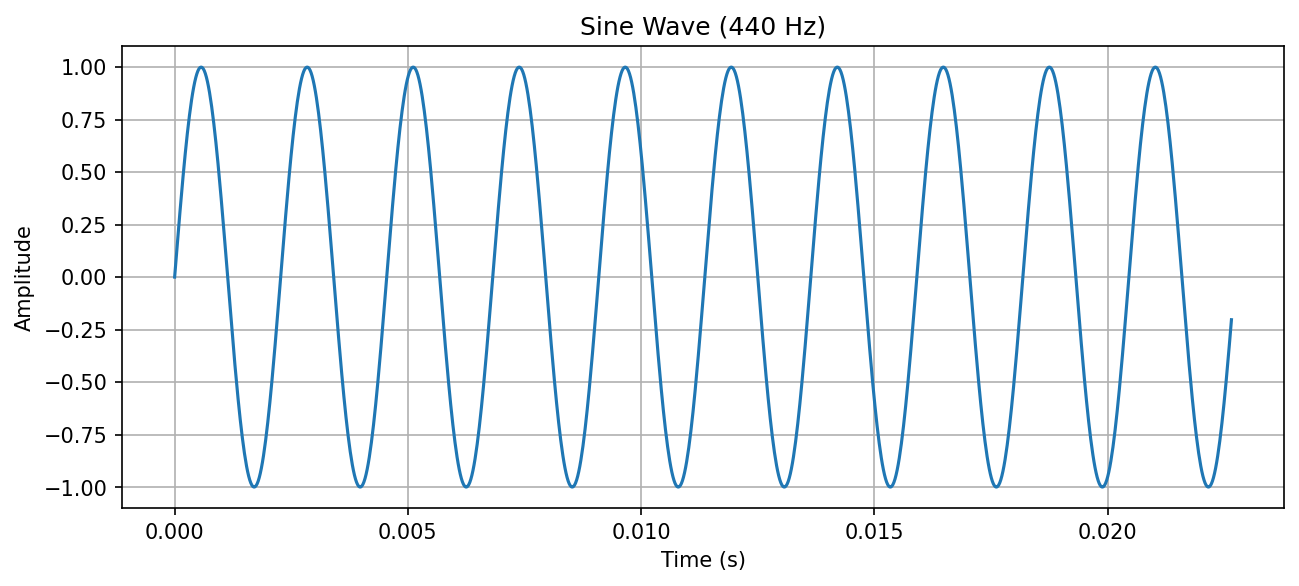
\includegraphics[width=\textwidth]{sine_wave_test.png}
    \caption{Audio Test - Sine Wave}
    \label{fig:sinewave}
\end{subfigure}
\hfill
\begin{subfigure}[b]{0.48\textwidth}
    \centering
    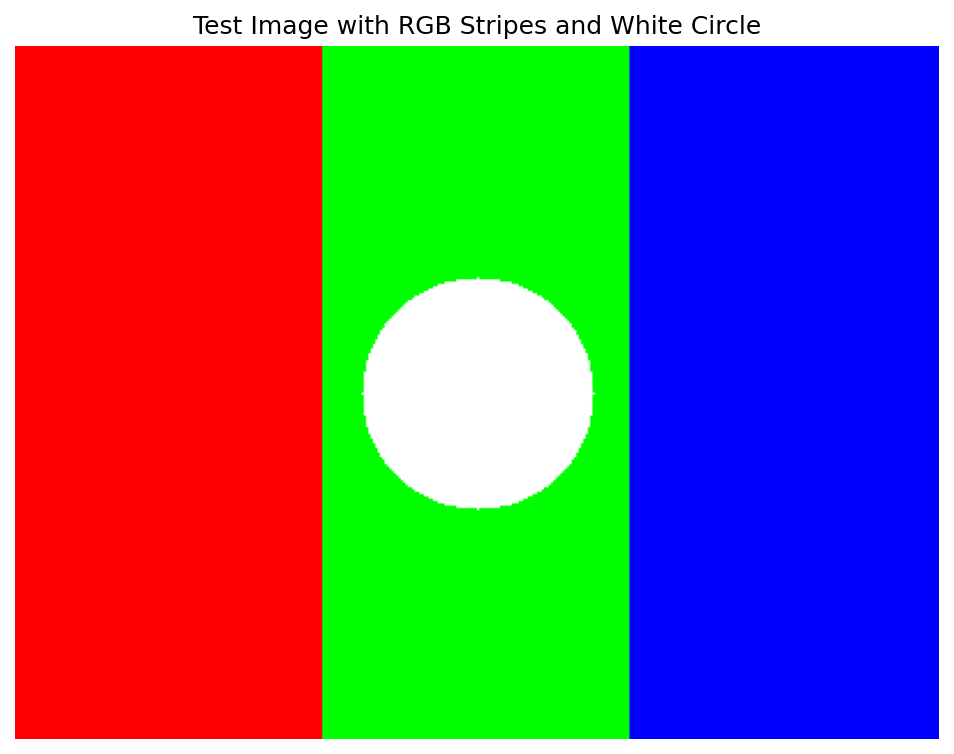
\includegraphics[width=\textwidth]{test_image.png}
    \caption{Image Test - RGB Pattern}
    \label{fig:testimage}
\end{subfigure}
\caption{Hasil Test Simple Code untuk Audio dan Image Processing}
\label{fig:test-results}
\end{figure}

\begin{figure}[h!]
\centering
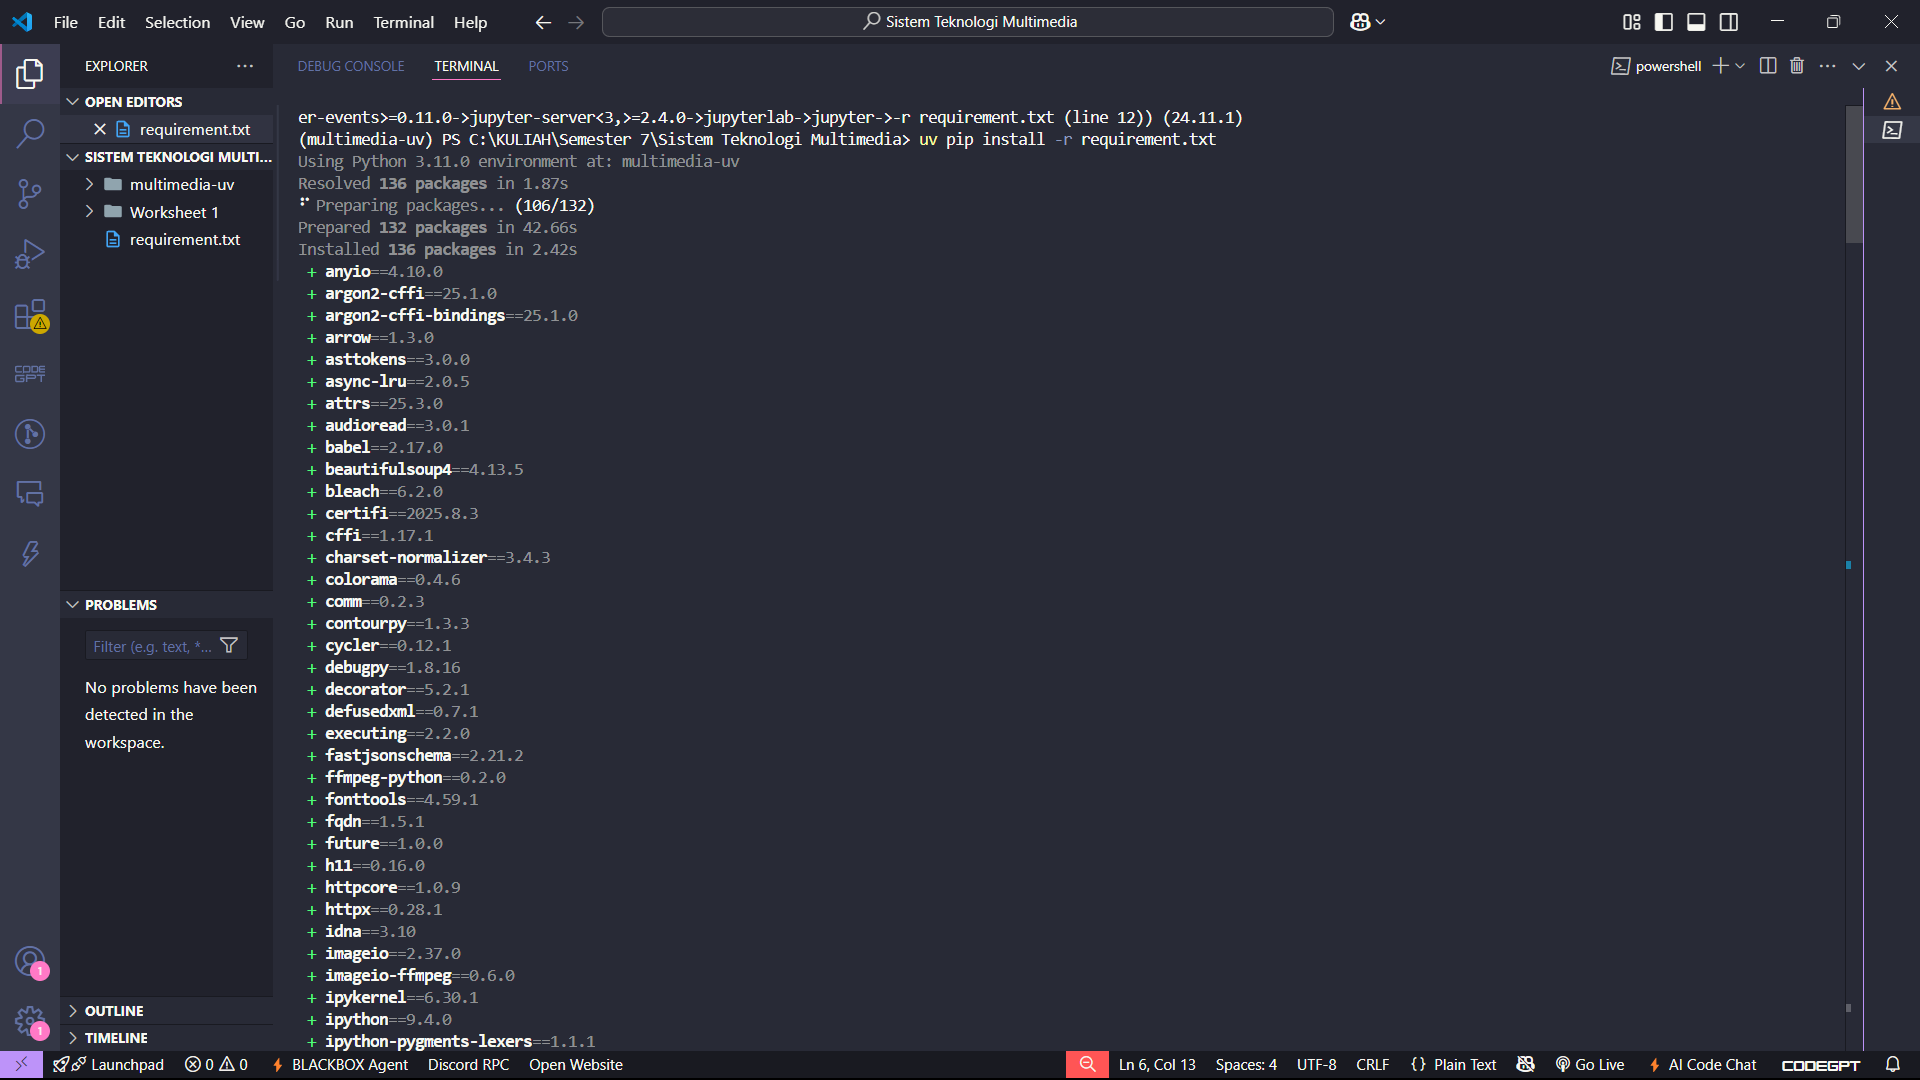
\includegraphics[width=0.8\textwidth]{figure/env.png}
\caption{Screenshot Environment Setup dan Import Test}
\label{fig:environment}
\end{figure}

\subsection{Analisis dan Refleksi}
\textbf{Jawab pertanyaan berikut:}

\begin{enumerate}
    \item \textbf{Mengapa penting menggunakan environment terpisah untuk project multimedia?}
    
    Environment terpisah sangat krusial untuk project multimedia karena library multimedia sering memiliki dependency yang kompleks dan spesifik. Misalnya, OpenCV membutuhkan versi NumPy tertentu, sedangkan librosa mungkin butuh versi berbeda. Tanpa environment terpisah, kita bisa mengalami konflik dependency yang membuat project tidak berjalan. Selain itu, multimedia project biasanya memerlukan library dengan ukuran besar seperti TensorFlow atau PyTorch, sehingga isolasi environment membantu menjaga sistem tetap bersih.
    
    \item \textbf{Apa perbedaan utama antara conda, venv, dan uv? Mengapa Anda memilih tool yang Anda gunakan?}
    
    \textbf{Conda} adalah package manager yang bisa mengelola binary dependencies, cocok untuk data science. \textbf{Venv} adalah built-in Python yang sederhana tapi hanya mengelola Python packages. \textbf{UV} adalah tool modern yang sangat cepat dalam resolving dependencies dan instalasi. Saya memilih UV karena kecepatannya yang luar biasa - instalasi library yang biasanya memakan waktu menit dengan pip bisa selesai dalam hitungan detik. Plus, UV memiliki dependency resolver yang lebih canggih sehingga mengurangi risiko konflik.
    
    \item \textbf{Library mana yang paling sulit diinstall dan mengapa?}
    
    MoviePy adalah library yang paling challenging karena memerlukan FFmpeg sebagai dependency eksternal. Di Windows, FFmpeg tidak otomatis terinstall dan perlu setup manual atau melalui package manager seperti chocolatey. Selain itu, OpenCV juga kadang bermasalah karena ada beberapa variant (opencv-python, opencv-contrib-python) yang bisa konflik. Librosa juga terkadang bermasalah di Windows karena dependency pada library audio backend seperti soundfile.
    
    \item \textbf{Bagaimana cara mengatasi masalah dependency conflict jika terjadi?}
    
    Langkah pertama adalah menggunakan \texttt{pip check} untuk mengidentifikasi konflik. Jika ada konflik, coba install versi spesifik yang kompatibel dengan \texttt{pip install package==version}. Alternatifnya, gunakan \texttt{pip-tools} atau \texttt{pipdeptree} untuk melihat dependency tree. Jika masih bermasalah, buat environment baru yang clean dan install library satu per satu sesuai prioritas. UV sangat membantu di sini karena dependency resolver-nya lebih pintar dalam menangani konflik dibanding pip biasa.
    
    \item \textbf{Jelaskan fungsi dari masing-masing library yang berhasil Anda install!}
    
    \textbf{Audio:} Librosa untuk analisis audio (spektogram, MFCC), SoundFile untuk I/O audio files, SciPy untuk signal processing. \textbf{Image:} OpenCV untuk computer vision dan image processing, Pillow untuk basic image operations, Scikit-image untuk advanced image processing algorithms. \textbf{Video:} MoviePy untuk editing dan manipulasi video, FFmpeg-python sebagai wrapper FFmpeg. \textbf{General:} NumPy untuk numerical computing, Pandas untuk data manipulation, Matplotlib untuk plotting dan visualization, Jupyter untuk interactive development environment.
\end{enumerate}

\subsection{Troubleshooting}
\textbf{Dokumentasikan masalah yang Anda hadapi (jika ada) dan cara mengatasinya:}

\begin{itemize}
    \item \textbf{Masalah 1:} MoviePy import error karena FFmpeg tidak ditemukan
    
    \textbf{Solusi:} Install FFmpeg secara manual atau gunakan \texttt{conda install ffmpeg} jika menggunakan conda. Untuk Windows, bisa download FFmpeg binary dan tambahkan ke PATH.
    
    \item \textbf{Masalah 2:} Librosa instalasi lambat karena building dari source
    
    \textbf{Solusi:} Gunakan pre-compiled wheel dengan \texttt{pip install --only-binary=all librosa} atau switch ke conda yang sudah menyediakan binary package.
\end{itemize}

\section{Export Environment untuk Reproduksi}
Sebagai langkah terakhir, export environment Anda agar dapat direproduksi:

\subsection{Untuk Conda}
\begin{lstlisting}[language=bash, caption=Export conda environment]
conda env export > environment.yml
\end{lstlisting}

\subsection{Untuk venv/uv}
\begin{lstlisting}[language=bash, caption=Export pip requirements]
pip freeze > requirements.txt
\end{lstlisting}

\textbf{Copy-paste isi file environment.yml atau requirements.txt di sini:}

\begin{lstlisting}[caption=Requirements.txt untuk UV Environment]
librosa==0.11.0          
soundfile==0.13.1        
scipy==1.16.1            
opencv-python==4.12.0.88 
pillow==11.3.0           
scikit-image==0.25.2     
matplotlib==3.10.5       
moviepy==2.2.1           
ffmpeg-python==0.2.0     
numpy==2.2.6             
pandas==2.3.2            
jupyter==1.1.1           

\end{lstlisting}

\section{Kesimpulan}
\textbf{Tuliskan kesimpulan Anda mengenai:}
\begin{itemize}
    \item Pengalaman setup Python environment untuk multimedia
    \item Persiapan untuk project multimedia selanjutnya
    \item Saran untuk mahasiswa lain yang akan melakukan setup serupa
\end{itemize}

Pengalaman setup Python environment untuk multimedia cukup menantang karena kompleksitas dependency antar library. UV terbukti sangat membantu dengan kecepatan instalasi yang luar biasa dan dependency resolution yang lebih baik dibanding pip. Environment yang sudah disiapkan ini memberikan foundation yang solid untuk project multimedia selanjutnya, dengan semua library utama (audio, image, video processing) sudah terintegrasi dengan baik.

Untuk mahasiswa lain, saya sarankan: 1) Selalu gunakan environment terpisah untuk setiap project, 2) Pertimbangkan UV untuk kecepatan dan reliability, 3) Test instalasi dengan script sederhana seperti yang sudah dibuat, 4) Dokumentasikan versi library yang digunakan untuk reproducibility, 5) Siapkan requirements.txt dari awal untuk memudahkan sharing dan deployment project.

\section{Referensi}
\begin{enumerate}
    \item LLM GPT \\
          \url{https://chatgpt.com/share/68aed053-1fec-800f-9a49-b502ec5eb92e}
    
\end{enumerate}
\end{document}